
\section{Results}
By using our proposed method, we pruned a four years old virtual
untrained tree (shown in Fig.~\ref{fig:my_figure4}) by using the proposed method and
compared the results to the pruning performed by horticulture expert.
The tree training teaching environment EduAPPLE \cite{kohek_eduapple:_2015} was used for
this purpose. The expert shaped the tree into two primary forms, a
pyramidal growing form HeP (Human expert - Pyramidal), which is similar to a Slender Spindle, and a
growing form HeF (Human expert - Flatt), suitable for the Fruiting Wall planting system. For
the automated pruning, we used a cone with the height of \(3\)m and the
opening angle of \(45{^\circ}\) (DDECn - DDE method, Conical initial shape), and a cylinder with a height of
3m and radius of 0.75 m (DDECy - DDE method, Cylindrical initial shape). In both cases, \(s_{\mathrm{\max}}\)
was set to 50. The pruning results can be seen in Fig.~\ref{fig:my_figure4}.
\begin{figure}[hbt]
    \centering
    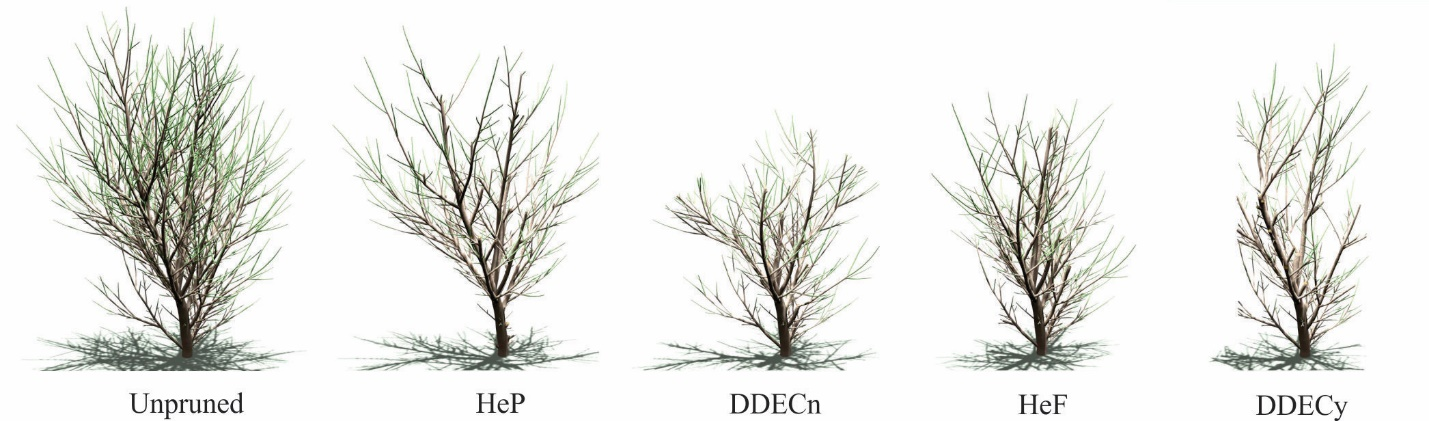
\includegraphics[width=5.4in]{figs/image4.jpeg}
    \caption{Comparison of pruning with the initial unpruned tree,
tree pruned by a human expert in a pyramidal shape (HeP), automated
pruning with initial cone shape (DDECn), pruning by human expert pruning
in a plat plane (HeF), automated pruning with the use of cylindrical
initial shape (DDECy).}
    \label{fig:my_figure4}
\end{figure}

In all four cases, the light distribution inside the tree crown is
significantly improved as compared to the unpruned tree (Fig.~\ref{fig:my_figure5}). In the unpruned
tree only 14.89 \% of buds receive more than 70 \% of available light while in the the human-pruned tree the amount of such buds increases to 26.80 \% (HeP) and to the 22.95 \% (HeF).
The light distributions of automated tree pruning are comparable with
that of human expert (25,93 \% for DDECn and 24.18 \% for DDECy). By comparing HeP to DDECn the result in the cases of human pruning is slightly better but in the case of HeF and DDECy the automated pruning achieved better result, althoug the difference in both casses is less than 1.3 \%. The difference between the DDE
and human pruning is also visible in the category of the internodes left
in the tree after the pruning.

By combining both results, it can be concluded, that the human expert
achieved similar bud light exposure with less biomass removed,
which is desirable since the higher number of internodes with
well-illuminated buds represent the higher potential for the yield of
both increased quality and quantity. Another metric is to compare the
percentage of buds in the tree crown receiving more than 40 \% of light
available. In this case, the difference between automated and human
pruning is 0.87 \%, in the case of HeP and DDECn and 6.86 \% by methods HeL and DDECy in the favour of the later.

\begin{figure}[hbt]
    \centering
    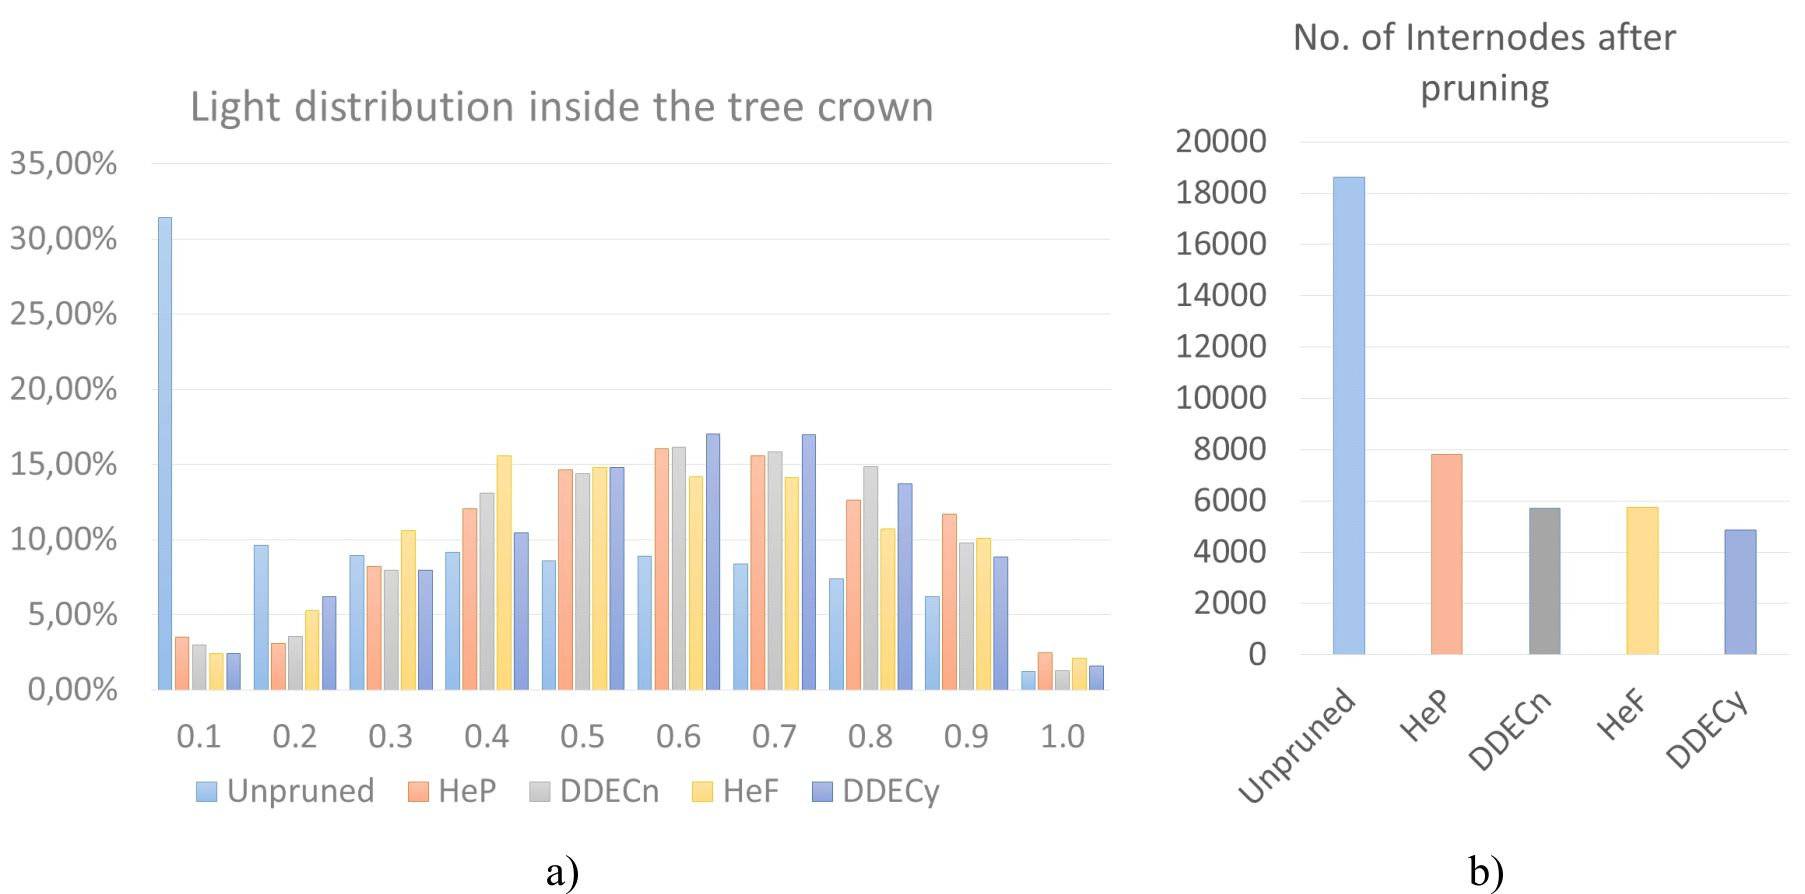
\includegraphics[width=5in]{figs/image5.jpeg}
    \caption{Evaluation of tree pruning results, a) Comparison of
light distribution after the pruning by a human expert (HeP and HeF) and
automated pruning (DDECn and DDECy), b) Number of internodes left after
the pruning. A higher number of internodes, combined with higher light
exposure of buds signify better results.}
\label{fig:my_figure5}
\end{figure}

DDECn and DDECy are representative of the selective pruning, where the
results of the first step represent the result of pruning by the
automatic pruning systems currently used. The difference between the
first and second step of DDECn and DDECy can be seen in Fig.~\ref{fig:my_figure6}.

\begin{figure}[hbt]
    \centering
    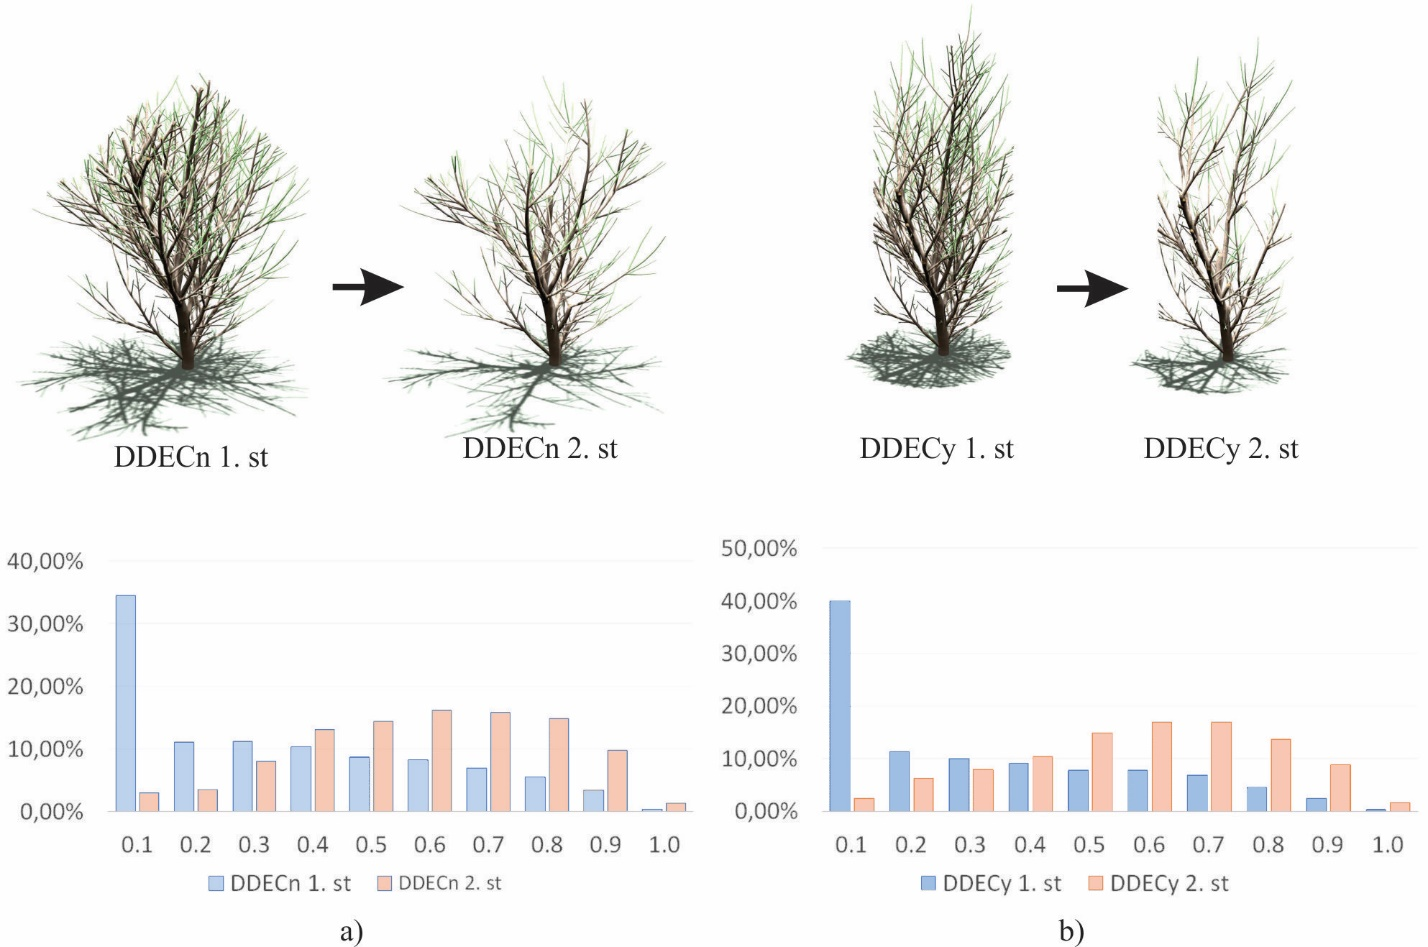
\includegraphics[width=5.4in]{figs/image6.jpeg}
    \caption{Tree crown light distribution after the first and
second pruning step, a) DDECn method, b) DDECy method}
    \label{fig:my_figure6}
\end{figure}

We also wanted to evaluate a long-term exposure to pruning and we were
curious if the proposed automated tree pruning method is capable of tree
training into desired growing form without human intervention. We have
simulated a row of five trees for six consecutive years. At the
beginning of each year, the trees were pruned by DDECn method to shape
them into the Slender Spindle growing form. The starting cone height was
1m and was linearly increased to 2.5m, which was the target height for
the trees in the following three years. The opening angle was constant
at 45° for the experiment duration. The initial value of the parameter
\(s_{\mathrm{\max}}\) was set to 20 and was linearly increased to 70 in
the sixth year. The result of the experiment can be seen in Fig.~\ref{fig:my_figure7}.

\begin{figure}[hbt]
    \centering
    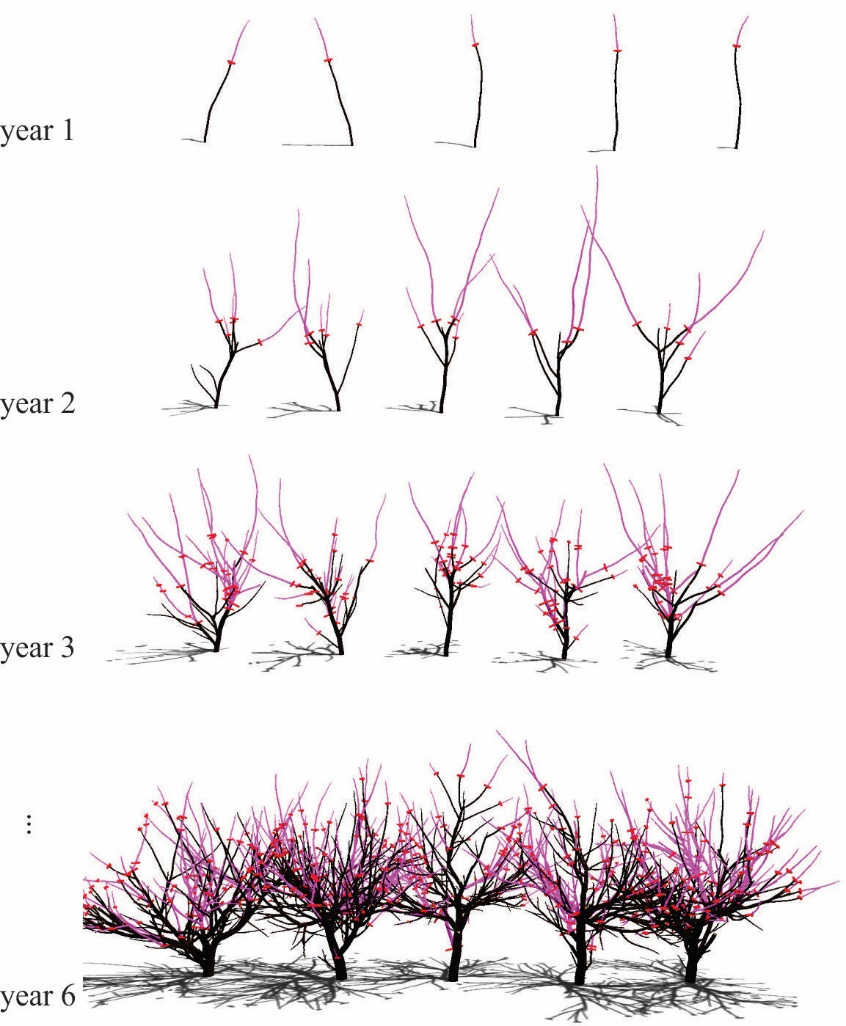
\includegraphics[width=3.84333in,height=4.66333in]{figs/image7.jpeg}
    \caption{Tree training of five apple trees into a Slender
Spindle growing form for six consecutive years with the DDECn method.
The purple color denotes removed branches}
    \label{fig:my_figure7}
\end{figure}


In general, as the tree structure becomes more complex in time, so the
value of \(s_{\mathrm{\max}}\ \)has to be increased. In our experiments,
we determined, that \(s_{\mathrm{\max}}\ \)should not exceed 150 even
for older trees.
